\documentclass[12pt,a4paper]{article}
\usepackage{math-text}
\usepackage{todonotes}
% \usepackage{multicol}
\usepackage{float}

\title{Хордовые диаграммы и ``инвариант Чмутова-Варченко''.\\ Заметки}
\author{Полина Закорко\and Глеб Минаев\and Саша Даниярходжаев\and Иван Русских}

\begin{document}
    \maketitle

    \listoftodos[TODOs]
    \par

    \vspace{2em}
    Написание этих заметок вдохновлено \href{https://mccme.ru/dubna/2021/courses/lando.html}{лекцией С.К. Ландо} на ЛШСМ 2021. В них мы записали (записываем) всё, что получили, изучая хордовые диаграммы, их графы пересечений и описанный в лекции ``инвариант Чмутова-Варченко''.

    \subsection{Краткий пересказ основных моментов лекции}

    \begin{definition}
        \emph{Хордовая диаграмма} --- набор из $n$ хорд на окружности, таких что
        \begin{itemize}
            \item концы хорд суть $2n$ попарно различных точек на окружности,
            \item концы хорд можно двигать по окружности, но нельзя их совмещать и менять их порядок.
        \end{itemize}
        Нас не будут интересовать геометрические составляющие чертёжа и конфигурации пересечений (пересекаются ли хорды в одной точке или нет), но будет интересовать, какие хорды пересекаются, а какие --- нет.

        \emph{Граф пересечений} хордовой диаграммы --- граф, вершины которого суть хорды данной хордовой диаграммы, а две вершины соединяются ребром тогда и только тогда, когда пересекаются соответствующие хорды.

        \emph{Инвариант Чмутова-Варченко} (для краткости также будем писать просто \emph{``инвариант ЧВ''} или \emph{``ИЧВ''}) --- многочлен, задаваемый хордовой диаграммой по следующим правилам (несложно понять по индукции, что ИЧВ всякой диаграммы определён):
        \begin{enumerate}
            \item \label{Chmutov-Varchenko-no-vertices} Инвариант ЧВ пустой диаграммы равен $1$.
                \begin{figure}[H]
                    \[
                        \raisebox{-35pt}{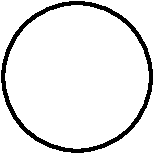
\includegraphics{images/ill.1.pdf}}
                        = 1
                    \]
                \end{figure}
            \item \label{Chmutov-Varchenko-empty-graph} Инвариант ЧВ диаграммы с ровно одной хордой равен $c$.
                \begin{figure}[H]
                    \[
                        \raisebox{-35pt}{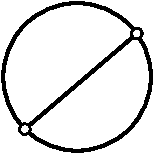
\includegraphics{images/ill.2.pdf}}
                        = c
                    \]
                \end{figure}
            \item \label{Chmutov-Varchenko-1-degree-vertex} При удалении ребра с ровно одним пересечением ИЧВ делится на $(c-1)$.
                \begin{figure}[H]
                    \[
                        \raisebox{-35pt}{\includegraphics{images/ill.30.pdf}}
                        = (c-1) \cdot
                        \raisebox{-35pt}{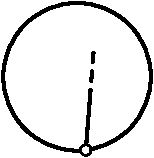
\includegraphics{images/ill.31.pdf}}
                    \]
                \end{figure}
            \item \label{Chmutov-Varchenko-connected-components} Диаграмма, состоящая из двух непересекающихся диаграмм, имеет ИЧВ, равный произведению ИЧВ данных диаграмм.
                \begin{figure}[H]
                    \[
                        \raisebox{-35pt}{\includegraphics{images/ill.40.pdf}}
                        =
                        \raisebox{-35pt}{\includegraphics{images/ill.41.pdf}}
                        \cdot
                        \raisebox{-35pt}{\includegraphics{images/ill.42.pdf}}
                    \]
                \end{figure}
            \item Также имеется два шестичленных правила-рекурренты.
                \begin{enumerate}
                    \item \label{Chmutov-Varchenko-monster-6-2} Первое правило.
                        \begin{figure}[H]
                            \[
                                \raisebox{-35pt}{\includegraphics{images/ill.20.pdf}}
                                =
                                \raisebox{-35pt}{\includegraphics{images/ill.21.pdf}}
                                +
                                \raisebox{-35pt}{\includegraphics{images/ill.22.pdf}}
                                -
                                \raisebox{-35pt}{\includegraphics{images/ill.23.pdf}}
                                +
                                \raisebox{-35pt}{\includegraphics{images/ill.24.pdf}}
                                -
                                \raisebox{-35pt}{\includegraphics{images/ill.25.pdf}}
                            \]
                        \end{figure}
                    \item \label{Chmutov-Varchenko-monster-6-3} Второе правило.
                        \begin{figure}[H]
                            \[
                                \raisebox{-35pt}{\includegraphics{images/ill.10.pdf}}
                                =
                                \raisebox{-35pt}{\includegraphics{images/ill.11.pdf}}
                                +
                                \raisebox{-35pt}{\includegraphics{images/ill.12.pdf}}
                                -
                                \raisebox{-35pt}{\includegraphics{images/ill.13.pdf}}
                                +
                                \raisebox{-35pt}{\includegraphics{images/ill.14.pdf}}
                                -
                                \raisebox{-35pt}{\includegraphics{images/ill.15.pdf}}
                            \]
                        \end{figure}
                \end{enumerate}
        \end{enumerate}
    \end{definition}

    Отметим важность следующей упомянутой на лекции теоремы.

    \begin{theorem}
        ИЧВ зависит только от графа пересечений. То есть, говоря формально, любые две диаграммы, имеющие одинаковый граф пересечений, имеют равные инварианты ЧВ.
    \end{theorem}

    Мы будем подразумевать её верность и использовать в дальнейшем. Также отсюда следует, что можно определять ИЧВ не только для хордовых диаграмм, но и для соответствующих им графов пересечений.

    В качестве мотивировки укажем, что одним из основных вопросов, поставленных на лекции, была следующая гипотеза.
    \begin{hypothesis}
        Пусть $p_n(c)$ --- ИЧВ полного графа на $n$ вершинах (или также хордовой диаграммы, получаемой проведением главных диагоналей вписанного $2n$-угольника), а
        \[P(c, t) := \sum_{n=0}^\infty p_n(c) t^n\]
        --- производящая функция данной последовательности. Тогда требуется показать, что
        \[
            P(c, t) =
            \dfrac{1}{
                1 - ct + \dfrac{ct^2}{
                    1 - (c-2)t + \dfrac{(4c-3)t^2}{
                        1 - (c-6)t + \dfrac{(9c-18)t^2}{
                            \dots + \dfrac{\mathstrut\cdots}{
                                1 - (c - n(n-1))t + \dfrac{(n^2 c - n^2(n^2 - 1))t^2}{
                                    \cdots
                                }
                            }
                        }
                    }
                }
            }
        \] 
    \end{hypothesis}
    Сложность гипотезы заключается как минимум в том, что сложность вычисления $p_n$ растёт экспоненциально быстро, и на данный момент посчитаны значения только для $n \leqslant 16$. На момент написания этих заметок гипотеза не доказана.

    \subsection{Частные результаты с применением компьютера}

    \begin{definition}
        Рассмотрим графы-циклы. Такие графы реализуются, например, $2n$-уголь\-ни\-ком с ребрами вида $(2k+1; 2k+4)$ ($k = 0, \dots, n-2$). Обозначим за $f_n$ инвариант ЧВ для цикла длины $n$, а $F := \sum_{n=0}^\infty f_n t^n$ --- производящая функция $f_n$.
    \end{definition}

    \begin{lemma}\ 
        \begin{enumerate}
            \item Верна рекуррента
                \[f_n = c (c-2) (c-1)^{n-2} + c f_{n-2} - f_{n-1}\]
                или по-другому
                \[f_n + f_{n-1} - c f_{n-2} = c (c-2) (c-1)^{n-2}.\]
            \item Верна формула
                \[f_n = (c-1)^n + \left(1 - \frac{2}{\sqrt{1+4c}}\right)\left(\frac{-1 - \sqrt{1+4c}}{2}\right)^n + \left(1 + \frac{2}{\sqrt{1+4c}}\right)\left(\frac{-1 + \sqrt{1+4c}}{2}\right)^n\]
            \item Верна формула
                \[F = \frac{3 - 2 (c-3) t - (4c-3) t^2}{(1 + t - ct)(1 + t - ct^2)}.\]
        \end{enumerate}
    \end{lemma}

    \begin{proof}\ 
        \begin{enumerate}
            \item Данная рекурента следует из применения \ref{Chmutov-Varchenko-monster-6-2} для случая $n > 3$ и \ref{Chmutov-Varchenko-monster-6-3} для случая $n = 3$.
            \item Несложно видеть, что
                \[
                    (f_n + f_{n-1} - c f_{n-2}) - (c-1)(f_{n-1} + f_{n-2} - c f_{n-3})
                    = c(c-2)(c-1)^{n-2} - (c-1)c(c-2)(c-1)^{n-3}
                    = 0
                \]
                Так мы получаем на последовательность $(f_n)_{n=0}^\infty$ линейную рекуренту с характеристическим многочленом
                \[(\lambda^2 + \lambda - c)\lambda - (c-1)(\lambda^2 + \lambda - c) = (\lambda^2 + \lambda - c)(\lambda - (c-1)).\]
                Если $\alpha$ и $\beta$ --- корни $\lambda^2 + \lambda - c$ (в частности, $\alpha + \beta = -1$, $\alpha \beta = -c$), то для некоторых $A$ и $B$
                \[f_n = C (c-1)^n + A\alpha^n + B\beta^n.\]
                Подставляя в изначальную рекуренту данную формулу, получаем $C = 1$. А $A$ и $B$ легко определить, подставляя $n = 0, 1$.
            \item Заметим, что рекуррента
                \[f_n + f_{n-1} - c f_{n-2} = c (c-2) (c-1)^{n-2}\]
                означает, что $F(c, t) \cdot (1 + t - c t^2)$ и $\sum_{n=0}^\infty c (c-2) (c-1)^{n-2} t^n$ совпадают во всех степенях $t$ кроме, быть может, 0 и 1. Следовательно
                \begin{gather*}
                    F(1 + t - c t^2) - (f_1 + f_0) t - f_0
                    = \sum_{n=2}^\infty c(c-2)(c-1)^{n-2} t^n\\
                    F(1 + t - c t^2) - (f_1 + f_0) t - f_0
                    = \frac{c(c-2) t^2}{(1 - (c-1)t)}\\
                    F(1 + t - c t^2)
                    = \frac{c(c-2) t^2}{(1 - (c-1)t)} + (f_1 + f_0) t + f_0\\
                    F(1 + t - c t^2)
                    = \frac{c(c-2) t^2}{(1 - (c-1)t)} + (c+3) t + 3\\
                    F(1 + t - c t^2)
                    = \frac{3 - 2 (c-3) t - (4c-3) t^2}{(1 + t - ct)}\\
                    F
                    = \frac{3 - 2 (c-3) t - (4c-3) t^2}{(1 + t - ct)(1 + t - ct^2)}
                \end{gather*}
        \end{enumerate}
    \end{proof}

    \begin{example}
        Если по рекуренте доопределить $f_0$, $f_1$ и $f_2$, то коэффициенты можно найти в следующей таблице (нули в таблице опущены).
        \begin{table}[H]
            \centering
            \begin{tabular}{c||c|c|c|c|c|c|c|c|c|c|c|c|c|c}
                $F$& $c^0$& $c^1$& $c^2$& $c^3$& $c^4$& $c^5$& $c^6$& $c^7$& $c^8$& $c^9$& $c^{10}$& $c^{11}$& $c^{12}$& $c^{13}$\\
                \hline
                \hline
                $f_0 = t^0$& 3&&&&&&&&&&&&&\\
                \hline
                $f_1 = t^1$&& 1&&&&&&&&&&&&\\
                \hline
                $f_2 = t^2$&&& 1&&&&&&&&&&&\\
                \hline
                $f_3 = t^3$&& 2& -3& 1&&&&&&&&&&\\
                \hline
                $f_4 = t^4$&& -4& 8& -4& 1&&&&&&&&&\\
                \hline
                $f_5 = t^5$&& 6& -13& 10& -5& 1&&&&&&&&\\
                \hline
                $f_6 = t^6$&& -8& 18& -18& 15& -6& 1&&&&&&&\\
                \hline
                $f_7 = t^7$&& 10& -23& 30& -35& 21& -7& 1&&&&&&\\
                \hline
                $f_8 = t^8$&& -12& 28& -48& 72& -56& 28& -8& 1&&&&&\\
                \hline
                $f_9 = t^9$&& 14& -33& 74& -133& 126& -84& 36& -9& 1&&&&\\
                \hline
                $f_{10} = t^{10}$&& -16& 38& -110& 225& -250& 210& -120& 45& -10& 1&&&\\
                \hline
                $f_{11} = t^{11}$&& 18& -43& 158& -355& 453& -462& 330& -165& 55& -11& 1&&\\
                \hline
                $f_{12} = t^{12}$&& -20& 48& -220& 530& -768& 926& -792& 495& -220& 66& -12& 1&\\
                \hline
                $f_{13} = t^{13}$&& 22& -53& 298& -757& 1238& -1727& 1716& -1287& 715& -286& 78& -13& 1\\
            \end{tabular}
        \end{table}
    \end{example}

    \begin{definition}
        Рассмотрим графы $K_{2,n}$ и $K_{1,1,n}$. Такие графы реализуются, например, $n$ параллельными рёбрами, которые пересекают два ребра, в случае $K_{2,n}$ параллельные и в случае $K_{1,1,n}$ пересекающиеся. Обозначим за $p_n$ и $q_n$ инвариант ЧВ для $K_{2, n}$ и $K_{1,1,n}$ соответственно, а $P := \sum_{n=0}^\infty p_n t^n$ и $Q := \sum_{n=0}^\infty q_n t^n$ --- их производящие функции.
    \end{definition}

    \begin{lemma}\ 
        \begin{enumerate}
            \item Верны рекурренты
                \[
                    p_{n+1} = (c-2) p_n - q_n + c^{n+2},
                    \qquad
                    q_{n+1} = (c-2) q_n - p_n + c^{n+2},
                \]
                или по-другому
                \[
                    p_{n+1} - (c-2) p_n + q_n = c^{n+2},
                    \qquad
                    q_{n+1} - (c-2) q_n + p_n = c^{n+2}.
                \]
            \item Верны формулы
                \begin{gather*}
                    p_n = \frac{1}{3} c^{n+2} + \frac{1}{6} c (4c-3) (c-3)^n + \frac{1}{2} c (c-1)^n\\
                    q_n = \frac{1}{3} c^{n+2} + \frac{1}{6} c (4c-3) (c-3)^n - \frac{1}{2} c (c-1)^n
                \end{gather*}
            \item Верны формулы
                \[
                    P = \frac{c^2 - (c^3-c^2-c)t - c^2 t^2}{(1-ct)(1-(c-1)t)(1-(c-3)t)},
                    \qquad
                    Q = \frac{(c^2-c) - (c^3-3c^2+2c)t - (c^3-2c^2)t^2}{(1-ct)(1-(c-1)t)(1-(c-3)t)}.
                \]
        \end{enumerate}
    \end{lemma}

    \begin{proof}\ 
        \begin{enumerate}
            \item Данная рекурента следует из применения \ref{Chmutov-Varchenko-monster-6-2} для случая $K_{2, n}$ и \ref{Chmutov-Varchenko-monster-6-3} для случая $K_{1,1,n}$ на двух данных и крайней хордах.
            \item Давайте рассмотрим $u_n := p_n + q_n$, $v_n := p_n - q_n$. Рассматривая сумму и разницу рекуррент, получаем
                \[
                    u_{n+1} - (c-3) u_n = 2 c^{n+2},
                    \qquad
                    v_{n+1} - (c-1) v_n = 0.
                \]
                В таком случае понятно, что $v_n = A (c-1)^n$, а переписывая рекуррентное соотношение на $u_n$ как
                \[(u_{n+2} - (c-3) u_{n+1}) - c(u_{n+1} - (c-3) u_n) = 0,\]
                получаем $u_n = B c^n + C (c-3)^n$. Подставляя $v_0$, имеем, что $A = c$. Подставляя $u_n$ в рекурренту
                \[u_{n+1} - (c-3) u_n = 2c^{n+2},\]
                получаем $B = \frac{2}{3}c^2$. Подставляя $u_0$, получаем $C = \frac{1}{3}c(4c-3)$. Таким образом по формулам
                \[p_n = \frac{u_n + v_n}{2} \qquad q_n = \frac{u_n - v_n}{2}\]
                восстанавливаются прямые формулы $p_n$ и $q_n$.
            \item В терминах предыдущего пункта введём $U = \sum_{n=0}^\infty u_n t^n$ и $V = \sum_{n=0}^\infty v_n t^n$ --- производящие функции нововведённых последовательностей. Очевидно, что
                \[U = P + Q, \qquad V = P - Q, \qquad \Longrightarrow \qquad P = \frac{U + V}{2}, \qquad Q = \frac{U - V}{2}.\]
                Рекуррента на $v_n$ означает, что
                \[V(1 - (c-1) t) - v_0 = 0,\]
                откуда
                \[V = \frac{v_0}{(1 - (c-1)t)} = \frac{c}{1 - (c-1)t}.\]
                Рекуррента на $u_n$ означает, что
                \begin{gather*}
                    U(1 - (c-3)t) - u_0
                    = \sum_{n=1}^\infty 2c^{n+2} t^n
                    = \sum_{n=0}^\infty 2c^{n+3} t^{n+1}
                    = \frac{2c^3 t}{(1-ct)}\\
                    U(1 - (c-3)t)
                    = \frac{2c^3 t}{(1-ct)} + c(2c-1)
                    = \frac{c(2c-1) + c^2 t}{(1-ct)}\\
                    U
                    = \frac{c(2c-1) + c^2 t}{(1-ct)(1-(c-3)t)}
                \end{gather*}
                Отсюда несложно понять искомый ответ.
        \end{enumerate}
    \end{proof}

    \begin{example}
        Коэффициенты $P$ и $Q$ можно найти в следующих таблицах (нули в таблицах опущены).
        \begin{table}[H]
            \centering
            \begin{tabular}{c||c|c|c|c|c|c|c|c|c|c|c|c}
                $P$& $c^0$& $c^1$& $c^2$& $c^3$& $c^4$& $c^5$& $c^6$& $c^7$& $c^8$& $c^9$& $c^{10}$& $c^{11}$\\
                \hline
                \hline
                $p_0 = t^0$&&&1&&&&&&&&&\\
                \hline
                $p_1 = t^1$&& 1& -2& 1&&&&&&&&\\
                \hline
                $p_2 = t^2$&& -4& 8& -4& 1&&&&&&&\\
                \hline
                $p_3 = t^3$&& 13& -30& 21& -6& 1&&&&&&\\
                \hline
                $p_4 = t^4$&& -40& 106& -96& 40& -8& 1&&&&&\\
                \hline
                $p_5 = t^5$&& 121& -362& 400& -220& 65& -10& 1&&&&\\
                \hline
                $p_6 = t^6$&& -364& 1212& -1572& 1070& -420& 96& -12& 1&&&\\
                \hline
                $p_7 = t^7$&& 1093& -4006& 5943& -4802& 2345& -714& 133& -14& 1&&\\
                \hline
                $p_8 = t^8$&& -3280& 13118& -21856& 20384& -11872& 4508& -1120& 176& -16& 1&\\
                \hline
                $p_9 = t^9$&& 9841& -42642& 78714& -83064& 56070& -25452& 7896& -1656& 225& -18& 1\\
            \end{tabular}

            \vspace*{10pt}
            \begin{tabular}{c||c|c|c|c|c|c|c|c|c|c|c|c|c|c}
                $Q$& $c^0$& $c^1$& $c^2$& $c^3$& $c^4$& $c^5$& $c^6$& $c^7$& $c^8$& $c^9$& $c^{10}$& $c^{11}$\\
                \hline
                \hline
                $q_0 = t^0$&& -1& 1&&&&&&&&&\\
                \hline
                $q_1 = t^1$&& 2& -3& 1&&&&&&&&\\
                \hline
                $q_2 = t^2$&& -5& 10& -5& 1&&&&&&&\\
                \hline
                $q_3 = t^3$&& 14& -33& 24& -7& 1&&&&&&\\
                \hline
                $q_4 = t^4$&& -41& 110& -102& 44& -9& 1&&&&&\\
                \hline
                $q_5 = t^5$&& 122& -367& 410& -230& 70& -11& 1&&&&\\
                \hline
                $q_6 = t^6$&& -365& 1218& -1587& 1090& -435& 102& -13& 1&&&\\
                \hline
                $q_7 = t^7$&& 1094& -4013& 5964& -4837& 2380& -735& 140& -15& 1&&\\
                \hline
                $q_8 = t^8$&& -3281& 13126& -21884& 20440& -11942& 4564& -1148& 184& -17& 1&\\
                \hline
                $q_9 = t^9$&& 9842& -42651& 78750& -83148& 56196& -25578& 7980& -1692& 234& -19& 1\\
            \end{tabular}
        \end{table}
    \end{example}

    % \subsection{Простые результаты}

    \subsection{Вариации начальной модели}

    Кроме всего нас также интересует как можно изменить модель так, чтобы в новых терминах искомые величины было легче изучать и/или вычислять на компьютере. Таким образом здесь мы приведём придуманные нами модели.

    \subsubsection{Модель с весами.}

    \todo[inline,color=green,caption={Написать про модель с весами.}]{
        Тут надо описать сашину модель, состоящую из:
        \begin{enumerate}
            \item графа пересечений,
            \item ``весов'' на вершинах графа, равных длине минимальной дуги, стягиваемой соответствующей хордой,
            \item ``весов'' на рёбрах графа, равных (ориентированному!) сдвигу одной дуги относительно другой (чтобы можно было точно восстановить их относительное положение). 
        \end{enumerate}
        Также для алгоритмической оптимизации можно попробовать хранить веса только в (на) остовном дереве.
    }

    \subsubsection{Модели на прямой.}

    \todo[inline,color=blue,caption={Написать про модели на прямой.}]{Их много, но эффекта не очень много. Надо попробовать, посмотреть, что получится.}

    \subsubsection{Модель на геометрическом графе.}

    \todo[inline,color=green]{Написать про модель на геометрическом графе.}

    % Пусть у нас есть какая-то хордовая диаграмма. Заметим, что
    % \begin{lemma}
    %     Следующие модели нативным образом переходят друг в друга:
    %     \begin{enumerate}
    %         \item хордовая $n$-диаграмма (т.е., с $n$ хордами),
    %         \item двумерный диск (или топологическое пространство, ему гомеоморфное), на котором проведены от края до края $n$ кривых, имеющие попарно не более одной общей точки, не имеющие общих концов и не имеющие потройно общих точек,
    %         \item окружность (или топологическое пространство, ему гомеоморфное), на котором выбраны $2n$ точек, разбитых на пары,
    %         \item хордовая $n$-диаграмма, где продолжения хорд находятся (геометрически) в общем положении,
    %         \item $n$ прямых общего положения в $\RR^2$ и замкнутая самонепересекающаяся кривая в общем положении с прямыми (т.е. не проходит через пересечения кривых).
    %         \item $n$ прямых общего положения в $\RR P^2$ и замкнутая самонепересекающаяся кривая в общем положении с прямыми (т.е. не проходит через пересечения кривых), вырезающая (с одной из сторон от себя) двумерный диск.
    %     \end{enumerate}
    %     \todo[inline]{Возможно, стоит дать определения построже?}
    % \end{lemma}
\end{document}